\documentclass[tikz,border=10pt]{standalone}
\begin{document}
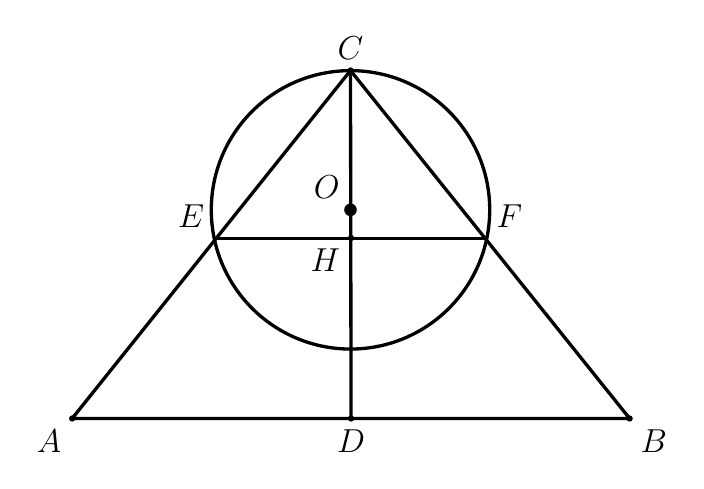
\begin{tikzpicture}[line width=1.2pt, line join=round]
% Coordinates: x=(px-305)*s, y=(213.5-py)*s, s=0.014981 cm/px
\coordinate (A) at (-3.557,-2.210);
\coordinate (B) at (3.523,-2.210);
\coordinate (C) at (-0.022,2.210);
\coordinate (D) at (-0.015,-2.210);
\coordinate (O) at (-0.022,0.440);
\coordinate (H) at (-0.015,0.082);
\coordinate (P6) at (-1.742,0.073);  % chord left end E, on circle
\coordinate (P5) at (1.697,0.073);   % chord right end F, on circle

% Circle (radius 118 px)
\draw (O) circle (1.768);

% Triangle and vertical altitude CD
\draw (A) -- (B) -- (C) -- cycle;
\draw (C) -- (D);

% Horizontal chord EF through H
\draw (P6) -- (P5);

% Small dots at labelled points (O handled separately, larger)
\foreach \p in {A,B,C,D,H}
  \fill (\p) circle (0.04);
% Filled centre dot, about 2x the others
\fill (O) circle (0.08);

% Labels
\node[above] at (C) {\fontsize{12}{14.4}\selectfont $C$};
\node[above left] at (O) {\fontsize{12}{14.4}\selectfont $O$};
\node[below left] at (H) {\fontsize{12}{14.4}\selectfont $H$};
\node[below left] at (A) {\fontsize{12}{14.4}\selectfont $A$};
\node[below] at (D) {\fontsize{12}{14.4}\selectfont $D$};
\node[below right] at (B) {\fontsize{12}{14.4}\selectfont $B$};
\node[above left] at (P6) {\fontsize{12}{14.4}\selectfont $E$};
\node[above right] at (P5) {\fontsize{12}{14.4}\selectfont $F$};
\end{tikzpicture}
\end{document}